

Voici le tableau de variations de la fonction $f$.

\begin{tikzpicture}
\tkzTabInit[lgt=1,espcl=2]{ $x$ / 1,$f $ / 2}
{ $-4$ , $-1$ ,1,5}
\tkzTabVar{-/$-5$,+/$3$,-/$-1$,+/$5$ }
\end{tikzpicture}
\begin{enumerate}
\item Comparer $f(2)$ et $f(4)$.
\item Trace une courbe qui représente cette fonction $f$.
\item Pour quelle valeur de $x$, $f(x)$ est minimal ? Que vaut ce minimum ?
\item Est-il vrai que $f(x)=0$ admet une solution ? Justifier.
\end{enumerate}